% Brett
\chapter{Experience with Kokkos}
\section{Performance}
Since Kokkos uses Cuda and OpenMP as a backend to achieve faster performance, we
chose to do some testing to confirm that Kokkos performs as well as these two
solutions. If Kokkos performed worse then Cuda or OpenMP, then programmers might
prefer these other solutions instead.  Fortunately, we found that Kokkos matches
the performance of Cuda and OpenMP in almost all cases.  The rest of this
section will describe our strategy for testing the performance of Kokkos
compared to Cuda and OpenMP, present graphs showing the differences observed,
and analyze the graphs.

In order to compare Kokkos, Cuda, and OpenMP, we wrote algorithmically
equivalent code using all three paradigms (using the same data layout and memory
access pattern) and recorded the runtime of each version.  To reduce noise in
the timing data, we repeated the same calculations five times and used the
average time.

Note that because we were unsure how Kokkos implements the intra-team \texttt{parallel\_reduce()}
function, we could not write a matching Cuda reduction.  Based on our project
priorities, we chose not to pursue this further.

These graphs present some of the performance differences and similarities of
Kokkos, Cuda, and OpenMP. Figure~\ref{fig:ContractDataDataScalar Kokkos
performance comparison} shows the raw times of Kokkos Cuda, Cuda, Kokkos OpenMP,
and OpenMP for \texttt{ContractDataDataScalar}.

\begin{figure}[!ht]
{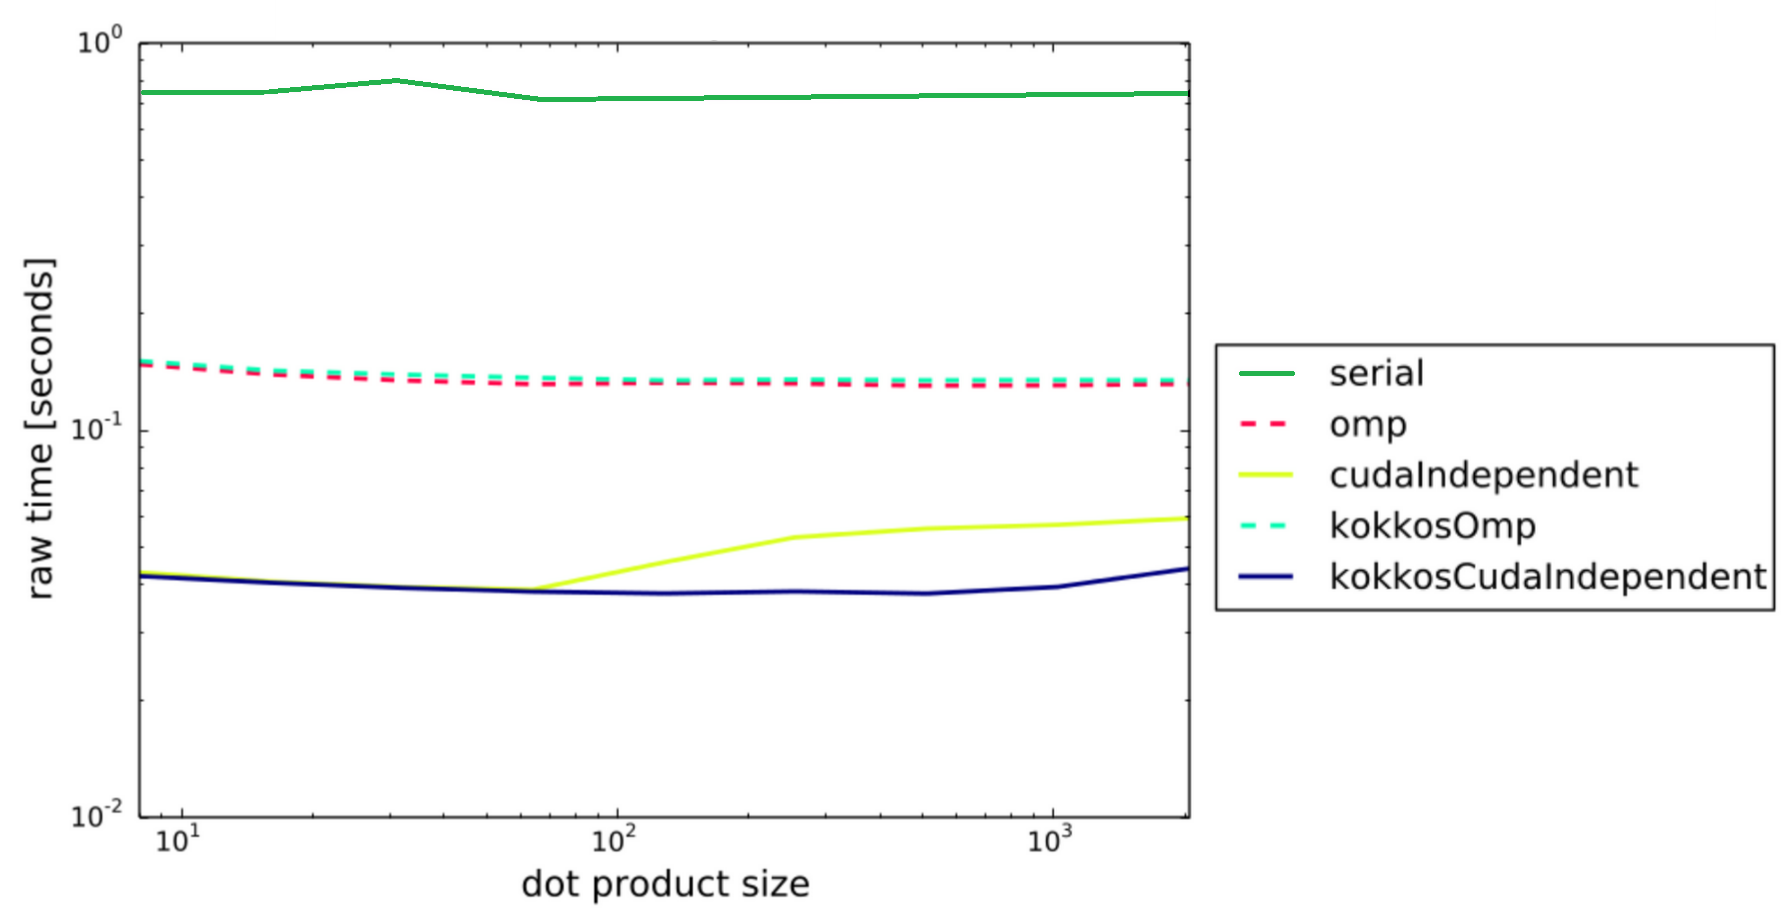
\includegraphics[scale=.7]{CDDS_FixedSerial.PNG}}
\caption[\texttt{ContractDataDataScalar} Kokkos performance comparison]{
    Performance of Kokkos Cuda, Cuda, Kokkos OpenMP,
and OpenMP for \texttt{ContractDataDataScalar} with a memory size of 1 GB.}
\label{fig:ContractDataDataScalar Kokkos performance comparison}
\end{figure}

In this graph, the $y$-axis is time in seconds, so closer to zero is better. The
$x$-axis plots different contraction sizes.  Here, Kokkos OpenMP and OpenMP are
almost perfectly overlapping. We are not quite sure why they are not perfectly
overlapping, but it appears too consistent to be random noise. However, the
difference is small enough as to be fairly insignificant. 

Kokkos Cuda, however, shows major differences compared to Cuda. The two perform
identically for the smaller problems but diverge by a significant amount for
bigger problems. This trend exists because Kokkos launches a different number of
blocks compared Cuda; Kokkos launches fewer blocks, with the intention of
reusing them.  We believe this doesn't affect small problem sizes because such
problems require fewer blocks than the large problem sizes, so both Kokkos and
Cuda launch enough blocks.  However, there is clearly a difference in the bigger
problem sizes. 

Figure~\ref{fig:cffscomparison} shows \texttt{ContractFieldFieldScalar} with the slicing
technique (which uses shared memory) for both Kokkos Cuda and Cuda.  It also
includes the flat parallel algorithm in both Kokkos Cuda and Cuda.

\begin{figure}[!ht]
{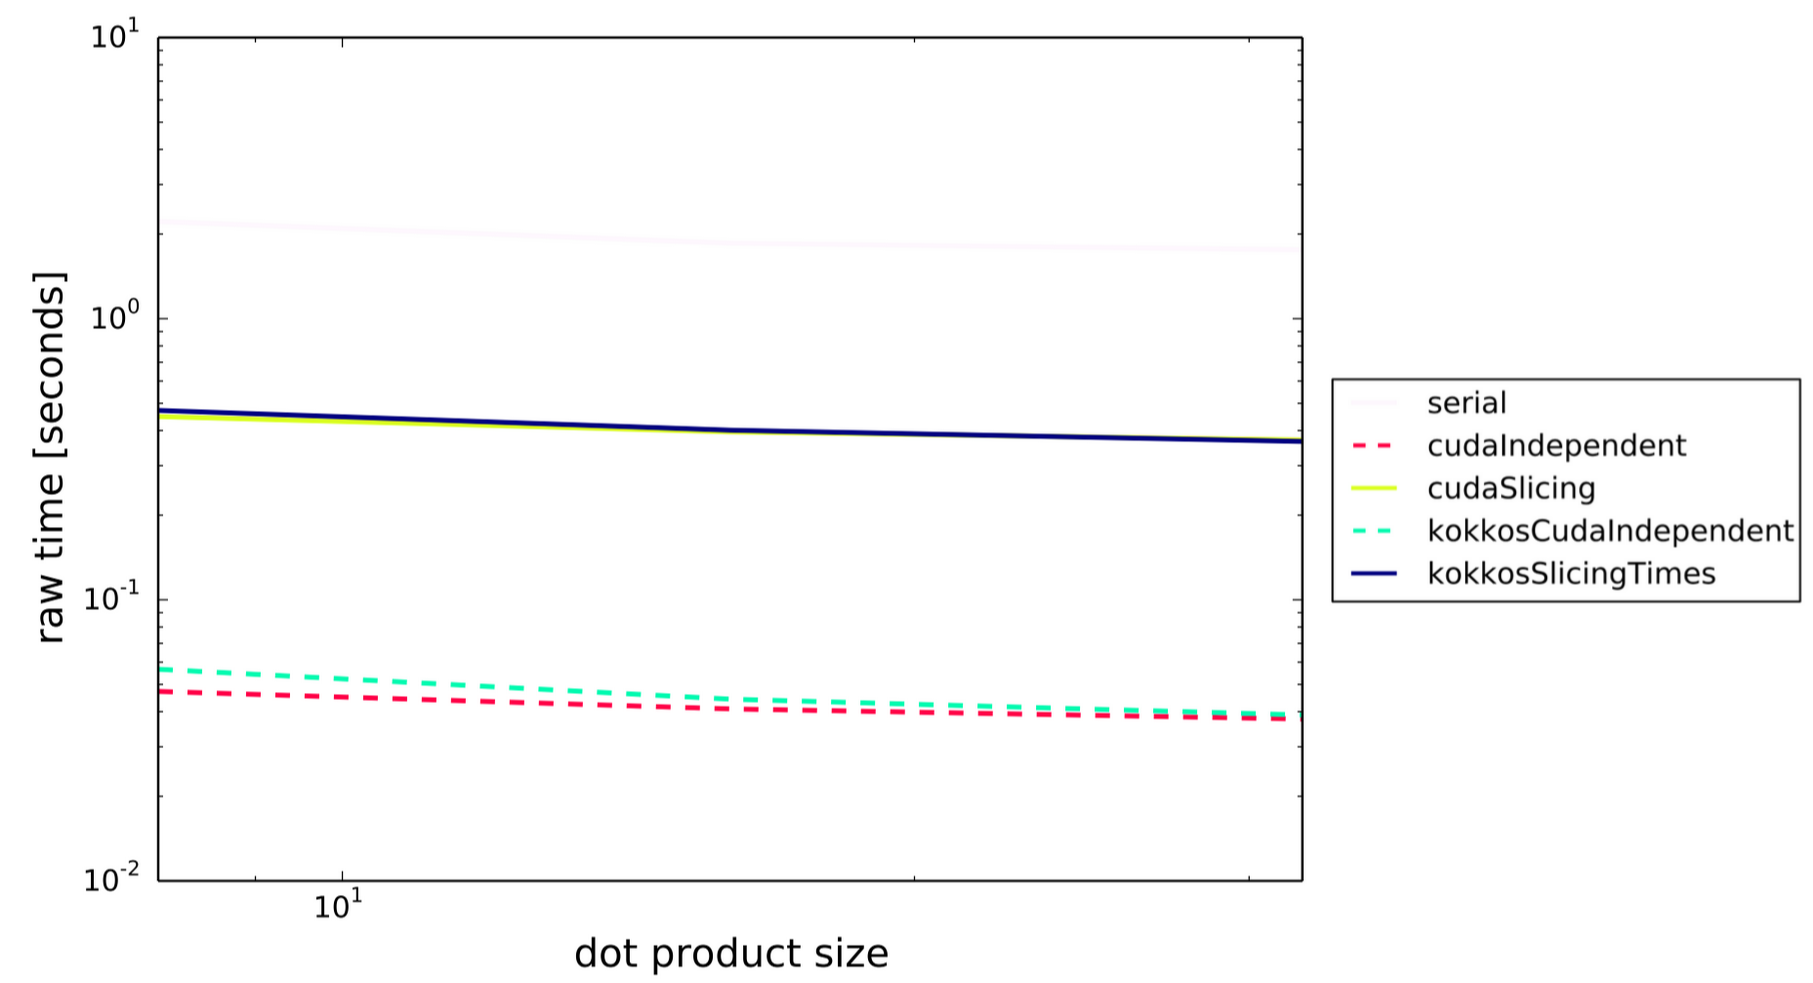
\includegraphics[scale=.8]{CFFS_RawTimes_LargestSize2.png}}
\caption[\texttt{ContractFieldFieldScalar} Kokkos performance comparison]{
    Performance of the ``slicing'' nested parallelism approach on \texttt{ContractFieldFieldScalar}.}
\label{fig:cffscomparison}
\end{figure}

In Figure~\ref{fig:cffscomparison}, the Cuda slicing performance is almost
identical to the Kokkos slicing performance. This shows that Kokkos' use of
shared memory matches that of Cuda.

Overall, most of our graphs show that Kokkos performs almost identically to Cuda
and to OpenMP.  We therefore concluded that Kokkos is not adding any major
overhead on a variety of problems. 
There may be slight performance differences due to optimization choices, but
Kokkos performs similarly to the native multithreading solutions.

\section{Code Snippets}
Another major factor that plays into whether programmers will use a language,
feature, or library is code complexity and ease of coding. Thus, we also
investigated the usability, readability, and intuitiveness of Kokkos compared to
Cuda and OpenMP.

Parallelizing code with Kokkos is significantly more complex than doing the same
with OpenMP.  However, OpenMP is considerably less flexible than Kokkos; it
works only on the CPU, and does not generalize to the GPU.  Therefore, in the
case of code that needs only to run on the CPU, we would strongly advise OpenMP
because of its simplicity.  However, that is not the niche that Kokkos is trying
to fill. 

Cuda, however, requires similar amounts of code to Kokkos.  The code snippets
presented will point out the differences and similarities directly.  First, we
will show the data setup step of moving data onto the GPU, and then move to
comparing and contrasting the Cuda kernel and the Kokkos functor.

Figure~\ref{lst:ContractFieldFieldScalar Cuda Data Setup} shows the setup of the data on the GPU for Cuda. 
There are three steps in the process: declaring a pointer to the data on the
CPU, allocating an array with the correct size on the GPU, then copying the data
over to the GPU from CPU (host) memory. This process is relatively simple and
self-explanatory. 
Equivalent Kokkos code is shown in Figure~\ref{lst:ContractFieldFieldScalar
Kokkos Cuda Data Setup}. Note that in a normal case, the data would already reside in the device View. The process in lines 12 - 25 is not necessary if the data is already on the device.

\begin{figure}[!htb]
	\begin{lstlisting}
float * leftDataArray = (...)	// Not shown populating data array
float * dev_leftDataArray;

cudaMalloc((void **) &dev_leftDataArray, 
	numContractions * numLeftFields * numPoints * 
	sizeof(float));
	
cudaMemcpy(dev_leftDataArray, &leftDataArray[0], 
	numContractions * numLeftFields * numPoints * sizeof(float), 
	cudaMemcpyHostToDevice);
	\end{lstlisting}

\caption{Code from Cuda \texttt{ContractFieldFieldScalar}
\label{lst:ContractFieldFieldScalar Cuda Data Setup}}
\end{figure}


\begin{figure}[!htb]
	\begin{lstlisting}
typedef Kokkos::Cuda	DeviceType;
typedef Kokkos::View<float***, Kokkos::LayoutRight, DeviceType>
	ContractionData;
typedef typename ContractionData::HostMirror
	ContractionData_Host;

ContractionData dev_ContractData_Left("left_data",
	numContractions,
	numLeftFields,
	numPoints);

ContractionData_Host contractionData_Left = 
	Kokkos::create_mirror_view(dev_ContractData_Left);

for (int cell = 0; cell < numContractions; ++cell) {
	for (int lbf = 0; lbf < numLeftFields; ++lbf) {
		for (int qp = 0; qp < numLeftFields; ++qp) {
			contractionData_Left(cell, lbf, qp) = 
				leftArray[cell*numLeftFields*
				numPoints + lbf*numLeftFields + qp];
		}
	}
}

Kokkos::deep_copy(dev_ContractData_Left, contractionData_Left);
	\end{lstlisting}
\caption{Code from Kokkos Cuda \texttt{ContractFieldFieldScalar}
\label{lst:ContractFieldFieldScalar Kokkos Cuda Data Setup}}
\end{figure}

The Kokkos code first defines and creates the device and host Views. One of the
major differences compared to Cuda is that Kokkos uses its own data structure, a
View, instead of an array. This requires typedefs to define the
Views, but the small amount of extra work gives the
programmer much more control over the data. The control also comes at the cost
of having to use loops to copy the data into the host view instead of simply
copying raw memory.

However, this initial work is done only once, and allows the user to change the
layout of the data by simply changing the \texttt{Kokkos::LayoutRight} to
\texttt{Kokkos::LayoutLeft}.  This is useful in optimizing the data layout for both the
CPU and GPU. Overall, Kokkos is more verbose, but also more abstract, as it must
perform on both the CPU and GPU while Cuda only runs on the GPU. 

In a program's computational portion, Cuda uses a kernel while Kokkos uses a
functor.  However, for programs doing the same calculation, the parenthesis
operator in a Kokkos functor is almost an exact replica of the code in
the corresponding Cuda kernel. A Cuda kernel for \texttt{ContractFieldFieldScalar} is
shown in Figure~\ref{lst:ContractFieldFieldScalar Cuda kernel}.

\begin{figure}[htb]
	\begin{lstlisting}
__global__ void
cudaContractFieldFieldScalar_Flat_kernel(int numContractions,
	int numLeftFields,
	int numRightFields,
	int numPoints,
	float * __restrict__ dev_contractData_Left,
	float * __restrict__ dev_contractData_Right,
	float * dev_contractResults) {
	int contractionIndex = blockId.x * blockDim.x + threadIdx.x;
	while (contractionIndex < numContractions) {
		int myID = contractionIndex;
		int myCell = myID / (numLeftFields * numRightFields);
		int matrixIndex = myID % (numLeftFields * 
			numRightFields);
		int matrixRow = matrixIndex / numRightFields;
		int matrixCol = matrixIndex % numRightFields;
		
		// Calculate now to save computation later
		int lCell = myMatrix * numLeftFields * numPoints;
		int rCell = myMatrix * numRightFields * numPoints;
		int resultCell = myMatrix * numLeftFields * 
			numRightFields;
		
		float temp = 0;
		for (int qp =0; qp < contractionSize; qp++) {
			temp += dev_contractData_Left[lCell + 
				qp*numLeftFields + matrixRow] *
				dev_contractData_Right[rCell + 
				qp*numRightFields + matrixCol];
		}

		dev_contractResults[resultCell + 
			matrixRow * numRightFields + matrixCol] = 
				temp;
		
		contractionIndex += blockDim.x * gridDim.x;
	}
}
	
	\end{lstlisting}
\caption{Code from Cuda \texttt{ContractFieldFieldScalar}
\label{lst:ContractFieldFieldScalar Cuda kernel}}
\end{figure}

The parenthesis operator in the corresponding Kokkos functor is shown in
Figure~\ref{lst:ContractFieldFieldScalar Kokkos Cuda functor}.

\begin{figure}[htb]
	\begin{lstlisting}
KOKKOS_INLINE_FUNCTION
void operator() (const unsigned int elementIndex) const {
	int myID = elementIndex;
	int myCell = myID / (_numLeftFields * _numRightFields);
	int matrixIndex = myID % (_numLeftFields * _numRightFields);
	int matrixRow = matrixIndex / _numRightFields;
	int matrixCol = matrixIndex % _numRightFields;

	float temp = 0;
	for (int qp = 0; qp < _numPoints; qp++) {
		temp += _leftFields(myCell, qp, matrixRow) *
			_rightFields(myCell, qp, matrixCol);
	}
	_outputFields(myCell, matrixRow, matrixCol) = temp;
}
	\end{lstlisting}
\caption{Code from Kokkos Cuda \texttt{ContractFieldFieldScalar}
\label{lst:ContractFieldFieldScalar Kokkos Cuda functor}}
\end{figure}

Although there are more lines of code in the Kokkos functor (the code required to
declare the data members and the constructor), the Kokkos code is readable and
uncluttered.

The Kokkos functor does not need to calculate each thread's location, while the Cuda
kernel has to use built-in constants such as \texttt{blockId.x} and \texttt{blockDim.x}.
Indexing into a View is easier than indexing into a primitive C-style array,
especially when changing the layout of the data between \texttt{LayoutLeft} and
\texttt{LayoutRight} because no code changes need to occur in the functor.

\section{Personal Experience and Thoughts}
\label{sec:Thoughts}

Part of our project's goal was to document our experiences using Kokkos,
including any issues we encountered.  As with any new tool or language, we
initially had some trouble getting used to Kokkos.  However, most of our initial
issues disappeared once we gained more experience with Kokkos.

Our liaison, Dr. Carter Edwards, installed Kokkos on our machine, so we are
unable to provide feedback regarding the process of downloading and installing
Kokkos.  We did, however, encounter some trouble in compiling and linking
against Kokkos. Our difficulties were mostly a consequence of insufficient or
outdated documentation of the compiler and linker flags Kokkos requires.  The
lack of documentation due to Kokkos' newness was a recurring problem for the
team.

Another obstacle we found was Kokkos' use of ``magic words''.  For example,
Kokkos requires the programmer to typedef \texttt{Kokkos::Cuda} or \texttt{Kokkos::OpenMP} to
\texttt{device\_type}; any other name would cause an error.  Though this is a simple line
to add, it is not an obvious requirement, and initially caused use some
confusion.  As with the compiler flags, formal documentation would have helped
in this situation; instead, we relied almost exclusively on example programs.
In Kokkos' favor, however, the fact that we were able to write all of our programs by
following a few examples shows Kokkos' intuitiveness.  Overall, we found Kokkos'
basic philosophy and structure to be elegant and well-designed.

The main difficulty the team encountered with Kokkos was its lack of
documentation.  While this is expected in a young project, poor documentation
made using Kokkos much more difficult.  We expect this to improve in the future,
making Kokkos significantly more attractive to users.

In addition, some planned and in-progress features of Kokkos will also be very
useful for future users. One example of such a feature is cartesian product
indexing for loops in Kokkos functors.  As we understand it, this feature will
allow users to specify multiple iteration indices, instead of just one, which
will remove the need for complicated arithmetic to extract the individual
indices from a single combined iteration index in multi-dimensional loops.  This
feature would have made our code much more concise and less prone to programmer
error.

As a whole, our team's experience with Kokkos has been positive.  It offers a
powerful, architecture-independent alternative to other multithreading
solutions.  Kokkos code is much easier to port between the CPU, GPU, and Xeon
Phi and Kokkos Views are powerful abstractions that allow a programmer to easily
change the layout of the data.  Kokkos functors are cleaner and more readable
than Cuda kernels, and the fact that Kokkos is a C++ library and not a new
language adds simplicity.  Changes we would like to see in Kokkos include View
layout options other than \texttt{LayoutRight} and \texttt{LayoutLeft} and the use of fewer
``magic words''.  Kokkos would also greatly benefit from more documentation as
well as better commenting in the example code.
